%%%%%%%%%%%%%%%%%%%%%%%%%%%%%%%%%%%%%%%%%
% LaTeX Template
% http://www.LaTeXTemplates.com
%
% Original author:
% Linux and Unix Users Group at Virginia Tech Wiki
% (https://vtluug.org/wiki/Example_LaTeX_chem_lab_report)
%
% License:
% CC BY-NC-SA 3.0 (http://creativecommons.org/licenses/by-nc-sa/3.0/)
%
%%%%%%%%%%%%%%%%%%%%%%%%%%%%%%%%%%%%%%%%%

%----------------------------------------------------------------------------------------
%	PACKAGES AND DOCUMENT CONFIGURATIONS
%----------------------------------------------------------------------------------------

\documentclass[12pt]{article}
\usepackage{geometry} % Pour passer au format A4
\geometry{hmargin=1cm, vmargin=1cm} %

\usepackage{graphicx} % Required for including pictures
\usepackage{float} %

%Français
\usepackage[T1]{fontenc}
\usepackage[english,francais]{babel}
\usepackage[utf8]{inputenc}
\usepackage{eurosym}
\usepackage{lmodern}
\usepackage{url}
\usepackage{multicol}

%Maths
\usepackage{amsmath,amsfonts,amssymb,amsthm}
%\usepackage[linesnumbered, ruled, vlined]{algorithm2e}
%\SetAlFnt{\small\sffamily}

%Autres
\linespread{1} % Line spacing
\setlength\parindent{0pt} % Removes all indentation from paragraphs

\pagestyle{empty}
\usepackage{lastpage}
\usepackage{fancyhdr} % Custom headers and footers
\pagestyle{fancyplain} % Makes all pages in the document conform to the custom headers and footers

\fancyfoot[C]{} % Page numbering for right footer
\fancyfoot[R]{\vspace{-1cm}\thepage / \pageref{LastPage}} % Page numbering for right footer



\renewcommand{\labelenumi}{\alph{enumi}.} %

%----------------------------------------------------------------------------------------
%	DOCUMENT INFORMATION
%----------------------------------------------------------------------------------------
\begin{document}

\setlength{\columnseprule}{0pt}

  \textsc{\LARGE Lycée Edouard Branly}\\[1.0cm] % Name of your university/college
  {\huge Durée de l'épreuve : 3 heures.}\\[0.5cm]

\noindent\hrulefill

\begin{center}
  \textsf{La normalité est une route pavée : on y marche aisément mais les fleurs n'y poussent pas. - Vincent Van Gogh}\\
\end{center}

\noindent\hrulefill

\begin{minipage}[t]{\textwidth}
  \raggedright
      {\bfseries BTS STS ET}\\
      {\bfseries Nom, Prénom : }\\[.35ex]
      \vspace*{-1cm}
      \raggedleft
          {\bfseries Devoir Bilan}\\[.35ex]
          {\bfseries 31 Mars 2015}\\[.35ex]
\end{minipage}\\[1em]

\noindent\hrulefill

\noindent\hrulefill

  \begin{minipage}{\textwidth}
    \begin{flushright} 
      Le sujet comporte $4$  pages numérotées de   $1/4$   à  $4/4$.\\
      Le sujet doit être rendu avec la copie à la fin de l’épreuve.\\
      Les 4 exercices à traiter sont indépendants.\\
      L'utilisation de la calculatrice est autorisée.\\
    \end{flushright}
  \end{minipage}


\section*{EXERCICE 1 - Fluctuation}



Soit $f$ la fonction définie sur $[-5 ; 5]$ par $f(x) = \dfrac{x}{2} * e^x$. On appelle $\mathcal{C}_f$ sa courbe représentative.

\begin{enumerate}
\item[1.] Démontrer que la fonction $f(x)$ n'est ni paire, ni impaire..
\item[2.] À l'aide d'une intégration par partie, calculer $\int_{0}^{4} f(x) dx$
\item[3.] À l'aide de votre calculette, tracer au mieux la fonction sur l'intervalle $[-5 ; 5]$.
\end{enumerate}

\begin{figure}[H]
  \centering
  \fbox{\includegraphics[width=0.8\textwidth]{sources/ie/grille-4.pdf}}
\end{figure}

\newpage
\section*{EXERCICE 2 - Flotte} % barème sur .
Une usine produit de l'eau minérale en bouteilles. Lorsque le taux de calcium  dans une bouteille est supérieur à 6.5mg par litre, on dit que l'eau de cette bouteille est calcaire.

\subsection*{Partie A - à la source}

L'eau minérale provient de deux sources : la source $A$ et la source $B$. On note $C$ l'événement : ``l'eau contenue dans la bouteille est calcaire''.

\begin{itemize}
\item La probabilité qu'une bouteille prélevée dans la production de la source A contienne de l'eau calcaire est 0.26. Soit $A$ l'événement : ``la bouteille provient de la source A''.
\item La probabilité qu'une bouteille prélevée dans la production de la source B contienne de l'eau calcaire est 0.15. Soit $B$ l'événement : ``la bouteille provient de la source B''.
\item La source $A$ produit $70\%$ de la production et la source $B$ le reste.
\end{itemize}

\begin{enumerate}
\item[1.]  Déduire du texte précédent les informations suivantes : $P(A)$, $P(B)$,  $P_A(C)$ et  $P_B(C)$
\item[2.] Calculer $P(C \cap A)$ et $P(C \cap B)$
\item[3.] En déduire $P(C)$
\item[4.] Calculer la probabilité que l'eau contenue dans une bouteille provienne de la source $A$ sachant quelle est calcaire.
\end{enumerate}

\subsection*{Partie B - à l'usine}

Dans un stock important de bouteilles $15\%$ contiennent de l'eau calcaire (on ne fait pas la distinction sur la provenance des bouteilles). On prélève au hasard 4 bouteilles dans le stock. On considère les tirages indépendants et avec remise. Soit X la variable aléatoire qui compte le nombre de bouteille avec de l'eau calcaire.

\begin{enumerate}
\item[1.]  Monter que cette situation correspond à une loi binomiale dont on précisera les paramètres.
\item[2.] Dessiner l'arbre de probabilité correspondant à la situation. Préciser le nombre de bouteilles avec l'eau calcaire à la fin de chaque branche.
\item[3.] Calculer la probabilité des événements suivants.
  \begin{enumerate}
  \item[a)] $D_0$ : ``Aucune des bouteilles ne contient de l'eau calcaire.
  \item[b)] $D_1$ : ``Il y a exactement une seule bouteille contenant de l'eau calcaire.
  \item[c)] $D_2$ : ``Il y a exactement deux bouteilles contenant de l'eau calcaire.
  \item[e)] $D_3$ : ``L'intégralité des trois bouteilles contient de l'eau calcaire.
  \end{enumerate}
\end{enumerate}

\newpage
\section*{EXERCICE 3 - Des jeux} % barème sur .

\subsection*{Partie A - Dés}

Un dé a été truqué.
\begin{itemize}
\item La probabilité de sortie du 5 est le double de la probabilité de sortie du 1. 
\item La probabilité de sortie du 6 est le triple de la probabilité de sortie du 1.
\item Les numéros 1, 2, 3 et 4 ont la même probabilité de sortie.
\end{itemize}

\begin{enumerate}
\item[1.] Donner le modèle de probabilité en calculant les probabilités de sortie de chaque numéro. On note $p_1$ la probabilité de faire 1, $p_2$ la probabilité de faire 2...
\item[2.] Calculer la probabilité de l'événement $A$ : ``Obtenir un numéro pair''.
\item[3.] Marge a obtenu le numéro 3. C'est à votre tour de jouer. Calculer la probabilité de l'événement $B$ : ``obtenir une face avec un numéro supérieur à celui de marge.''
\end{enumerate}


\subsection*{Partie B - Motus}

Une fête réunit $25$ hommes, $100$ femmes, $25$ enfants. Sur une table, il y a $3$ urnes : $H$, $F$, $E$ contenant des boules de couleurs dont respectivement $10\%$, $40\%$, $80\%$ de boules noires. On note $B$ l'événement : ``la boule tirée est noire''.\\
Un présentateur aux yeux bandés désigne une personne au hasard et lui demande de tirer une boule dans l’urne $H$ si cette personne est un homme, dans l’urne $F$ si cette personne est une femme, dans l’urne $E$ si cette personne est un enfant.

\begin{enumerate}
\item[1.] Déduire du texte précédent les informations suivantes : $P(H)$, $P(F)$ et 
$P(E)$.
\item[2.] Déduire du texte précédent les informations suivantes : $P_H(B)$, $P_F(B)$ et $P_E(B)$.
\item[3.] Calculer $P(B \cap H)$, $P(B \cap F)$ et $P(B \cap E)$.
\item[4.] Quelle est la probabilité que la boule tirée soit noire.
\end{enumerate}

\subsection*{Partie C - Carte}

Dans un jeu de 52 cartes, il y a des piques, des cœurs, des trèfles et des carreaux. Les cartes sont numérotés de 1 à 10 puis valet, dame et roi.\\
On tire une carte au hasard dans ce jeu.

\begin{itemize}
\item Soit $A$ l'événement : ``la carte tirée est un AS''.
\item Soit $C$ l'événement : ``la carte tirée est un cœur''.
\end{itemize}

\begin{enumerate}
\item[1.] Calculer les probabilités $P(A)$ et $P(C)$.
\item[2.] Définir par une phrase l'événement $\overline{A}$ puis calculer $P(\overline{A})$. 
\item[3.] Définir par une phrase l'événement $A \cap C$ puis calculer $P(A \cap C)$. 
\item[4.] Définir par une phrase l'événement $A \cup C$. Déduire des questions précédentes $P(A \cup C)$. 
\end{enumerate}

\newpage
\section*{EXERCICE 4 - Étude de fonction} % barème sur .

Soit $f$ la fonction définie sur $\mathbb{R}$ par $f(x) = -2e^{x} + 8$. On appelle $\mathcal{C}_f$ sa courbe représentative.

\setlength{\columnseprule}{1pt}
\begin{multicols}{2}

\subsection*{Partie A - Dérivée}

La fonction est dérivable sur $\mathbb{R}$ et on appelle $f'(x)$ sa fonction dérivée.

\begin{enumerate}
\item[1.] Déterminer $f'(x)$ pour tout $x$ réel.
\item[2.] Étudier le signe de $f'(x)$ sur $\mathbb{R}$.
\item[3.] En déduire les variations de $f(x)$ sur $\mathbb{R}$.
\end{enumerate}

\subsection*{Partie B - Limites}

\begin{enumerate}
\item[1.] Déterminer la limite de $f$ lorsque $x$ tend vers $+\infty.$
\item[2.] Déterminer la limite de $f$ lorsque $x$ tend vers $-\infty.$
\item[3.] La courbe $\mathcal{C}_f$ admet une asymptote. En déduire son équation.
\end{enumerate}

\end{multicols}

\subsection*{Partie C - Courbe et Intégrale}

\begin{enumerate}
\item[1.] Tracer la courbe représentative $\mathcal{C}_f$ de la fonction $f$.
\item[2.] Sur le graphique suivant, indiquer en coloriant (ou hachurant) à quoi correspond l'intégrale :  $\int_{-3}^{0} f(x) dx$.
\item[3.] Sans l'aide des formules d'intégrations, on se propose de trouver ce résultat.
  \begin{enumerate}
  \item[a)] Donner les valeurs de $f(-3)$ et $f(0)$ en arrondissant à $10^{-2}$.
  \item[b)] Placer les points $A\left(-3, 0\right)$, $B\left(0, 0\right)$, $C\left(0, f(0)\right)$, $D\left(-3, f(0)\right)$ et $E\left(-3, f(-3)\right)$ sur le graphique.
  \item[c)] Calculer l'aire du rectangle $ABCD$ et l'aire de triangle $CDE$. En déduire une valeur approchée de l'intégrale $\int_{-3}^{0} f(x) dx$.
  \end{enumerate}   
\item[4.] Déterminer $F(x)$ une primitive de $f$ sur $\mathbb{R}$.
\item[5.] Calculer l'intégrale $\int_{-3}^{O} f(x) dx$.
\end{enumerate}

\begin{figure}[H]
  \centering
  \fbox{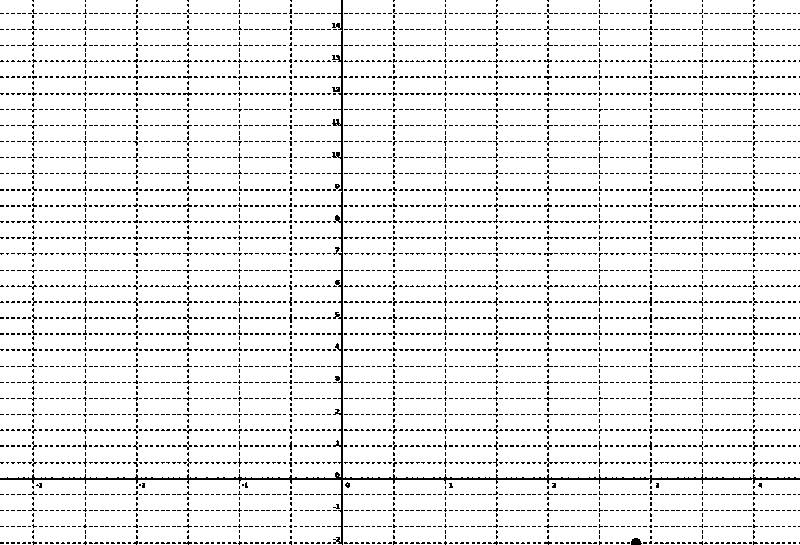
\includegraphics[width=0.8\textwidth]{sources/ie/grille-2.pdf}}
\end{figure}

\end{document}
